\chapter{Internal Electrode Sensitivity}
\label{chap:chapter-6}
\emph{This sensitivity analysis work has
 been presented in part at: the 42nd Annual International Conference of the IEEE Engineering 
 in Medicine \& Biology Society (EMBC 2020) \parencite{stowe_effect_2020}.} 

\section{Introduction}
Currently, the most common implementations of EIT in biomedical applications
measure voltages and inject currents from the body surface using 
one or two planes of electrodes. Internal electrodes are not used clinically
despite promising simulation studies that have shown large improvements 
in reconstruction accuracy and internal sensitivity in 
2D \parencite{nasehi_tehrani_evaluation_2012,nasehi_tehrani_modelling_2012}. 
In practice, EIT images with internal electrodes are challenging 
to interpret 
as the measurements are prone to errors 
due to probe 
plecement \parencite{czaplik_application_2014}. 

As discussed in \fref{chap:chapter-3}, one of the main challenges 
in perfusion imaging is the large difference in amplitude 
between the ventilation and cardiac signals. 
When using external electrodes, the respiratory amplitude is 
significantly larger than the cardiac component. 
Techniques such as 
breath holds, induced apnoea \parencite{leathard_comparison_1994,stowe_comparison_2019}, 
or injection 
of a contrast agent \parencite{frerichs_regional_2002} can reduce the
impact of the respiratory signal, but they are not feasible for 
long-term or continuous monitoring. 
Other methods such as averaging a large number of signals together 
have been used \parencite{eyuboglu_vivo_1989,vonk-noordegraaf_pulmonary_1998}, 
but as discussed by \citeauthorandyear{deibele_dynamic_2008} 
these do not allow real-time monitoring and 
may miss sudden changes in perfusion.
Filtering techniques have been implemented to help isolate the 
cardiac component of the signal, but there is occasionally overlap between 
the carsiosynchronous component and harmonics of the ventilation
signal. This makes signal separation more 
challenging \parencite{zadehkoochak_pulmonary_1992,leathard_comparison_1994}.
%Low sensitivity in central regions relative to the boundary
%limits the clinical applications of EIT. 

%Low sensitivity in the centre of 

%the model reduces the ability to
%accurately reconstruct and identify impedance changes  to
%the heart.

Internal electrodes have been proposed several times as a method to 
sustainably increase sensitivity in central regions of the 
chest and improve EIT reconstruction 
accuracy \parencite{pilkington_utilization_1989,schuessler_utility_1995,nasehi_tehrani_evaluation_2012, 
czaplik_application_2014,nguyen_electrical_2020}.
Past research in 2D identified a sixfold increase in the cardiac frequency 
component of the EIT signal 
when 2 of 16 total electrodes were placed in the 
esophagus or trachea compared to a typical external configuration
\parencite{czaplik_application_2014}. However, tt is not clear whether 
the identified increase in cardiac-frequency amplitude stems from pulsatile 
(motion-based), changes or whether these changes represent 
perfusion.

There is potential for clinical use of internal electrodes 
to monitor ventilation, perfusion and 
hemodynamic changes in the 
intensive-care unit (ICU), where patients typically have
breathing and feeding tubes in place.
EIT applications in development include mechanical ventilation 
guidance and monitoring \parencite{frerichs_chest_2017}, perfusion 
monitoring \parencite{frerichs_regional_2002,smit_electrical_2003}, 
blood pressure monitoring \parencite{sola_non-invasive_2011,proenca_noninvasive_2017}, 
and cardiovascular output \parencite{braun_accuracy_2018}. 
For all of these uses of EIT, internal sensitivity in the centre of 
a model could provide increased accuracy. 
In an 
intensive-care environment where feeding and breathing tubes 
are used, internal electrodes could provide 
several advantages without additional invasiveness. 
It has even been suggested that internal electrodes may replace 
electrodes on the back, which are challenging to place for critically 
ill patients who cannot be safely or easily 
moved \parencite{czaplik_application_2014}.
Internal electrodes placed in both the esophagus and the trachea
have been used, and both have shown increased sensitivity to cardiosynchronous
EIT signals \parencite{czaplik_application_2014}. 
Esophageal electrodes may be slightly easier to implement 
clinically as there are less hygiene concerns.

Especially while monitoring perfusion where one of the main challenges
has been the small amplitude of the cardiac signal,
\parencite{nguyen_review_2012}, internal electrodes offer
potential for improvement.
This chapter presents a 3D EIT configuration with internal electrodes
that can be used to maintain a high sensitivity in regions with 
large pulsatile components in the centre of a model.

Some studies have suggested different current injection and measurement patterns
to improve sensitivity when using internal electrodes \parencite{nasehi_tehrani_modelling_2012}.
This chapter presents a comparison between
an electrode injection pattern to increase
internal sensitivity to the standard ``skip 4''
measurement and injection pattern used in 3D.

The sensitivity benefits of internal electrode imaging in 3D are assessed
in simulation to determine the feasibility of using internal electrodes 
to improve perfusion monitoring. 
We expect to see that internal electrodes increase sensitivity in 3D configurations 
as they do in 3D.
This chapter provides proof of principle for internal electrode configurations 
in 3D to 
improve EIT sensitivity.

%The goal of this chapter is to determine the viability of internal 
%electrode use through a series of simulations and phantom measurements.
%We expect to show that using internal electrodes increases the 
%sensitivity of the measurements to internal impedance changes 
%and enables a higher resolution of image reconstructions in 
%these central regions of the thorax. 

\section{Methods}

\subsection{Tank Model}
This section exmpalins the techniques used to 
generate 3D meshes with different external and internal 
electrode configurations on a tank model. 
different numbers of electrode were added to visualize the sensitivity increase 
and determine if accurate constructions were feasible. 
To analyze the sensitivity changes due to different electrode 
configurations finite element models (FEMs) of a cylindrical tank were 
created with each of the tested electrode configurations. \Fref{fig:tank_FEM} shows the four 
different configurations that were tested: a 2D 
electrode ring of 32 electrodes; a 3D configuration of 2 layers of 16 
electrodes (3D(a)); a second 3D configuration of 2 layers of 15 electrodes 
plus 2 central internal electrodes inline with the electrode planes (3D(b)); and a final 3D configuration of 
2 layers of 14 electrodes with 4 central internal electrodes evenly spaced between the electrode planes (3D(c)).

\begin{figure}[H]
\centering
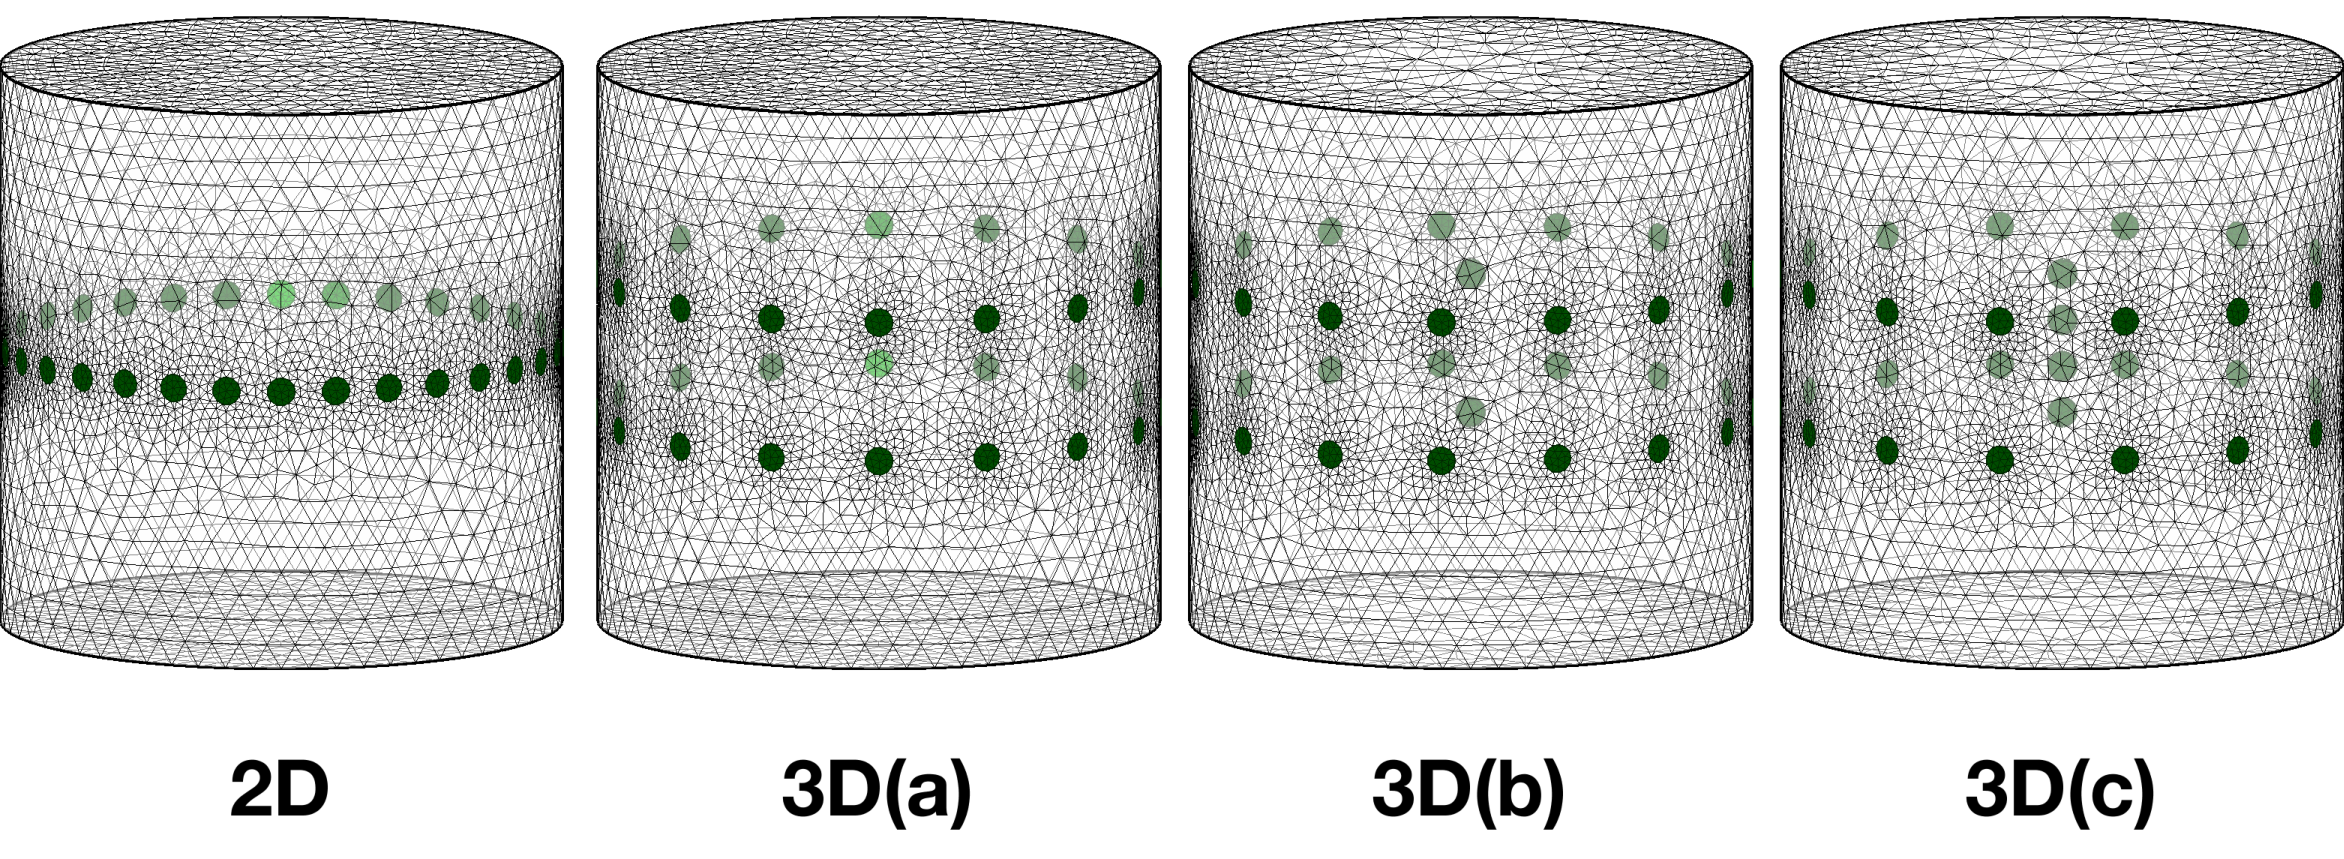
\includegraphics[width=\textwidth]{chapter6-internal_electrodes/imgs/FEM_Comparison.pdf}
\caption[Internal electrode configurations]{4 configurations of electrodes were tested: 2D) a single ring of 32 electrodes; 
	3D(a) 2 rows of 16 external electrodes; 3D(b) 2 rows of 15 external electrodes with 2 internal electrodes; and 3D(c) 2 rows 
of 14 external electrodes and 4 internal electrodes.}
\label{fig:tank_FEM}
\end{figure}

The tank in the simulations has a height of 2 m, radius of 1 m, and the electrode radius
is 0.05 m for both the round external electrodes and the spherical internal electrodes.
In the 3D configurations, the plane separation is 0.5 m and in all configurations the radial
spacing between electrodes is equal.
The background conductivity of the tank was 1 S/m and the conductivity of the target was
10 S/m.

When reconstructing images a conductive target was added to the tank
at a height of 1 m at the midpoint of the tank radius. The target
object radius is 0.4 m.

\subsection{Image Reconstruction}

To generate EIT images from voltage measurements, the 3D GREIT
reconstruction algorithm
was used \parencite{grychtol_3d_2016}. A spherical
conductive target with a radius of 20\% of the tank radius
was placed midway between the centre and boundary
of the tank, in a region with typically low sensitivity.
The inverse problem hyperparameter
was selected so that in all instances the amount of measurement
noise that propagated from the measurements into the final images
was equal. 500 training targets with a size of 5 cm were placed within the model to train the GREIT 
algorithm. 

\subsection{Sensitivitiy Calculation}

The sensitivity is then calculated from the jacobian ($J$) of the reconstruction matrix as:
\begin{equation}
	S = \frac{\sqrt{\sum_{i}\vec{J}_{ij}^2}}{V_i}
\end{equation}
where $V_i$ is the volume of each respective voxel. 

\subsection{Current Injection and Measurement}
For this analysis external electrodes are placed in 
a ``square'' pattern \parencite{grychtol_3d_2016} 
and the internal electrodes are placed from top to 
bottom. 

The current injection pattern used in this analysis was the 
typical ``skip 4'' injection pattern that has been shown to yield 
a good sensitivity distribution in 3D EIT \parencite{grychtol_3d_2016}.
A new stimulation and measurement pattern is also used in a model with 
two internal electrodes that increases
the number of measurements on the internal probe. This stimulation 
pattern is consistent with the skip 4 pattern, but 
for the measurements, every second measurement
is replaced with a measurement between the boundary and the internal probe. 
This results in the same total number of measurements, but many more measurements
use the internal probe. This new stimulation pattern is described in \fref{fig:modified_measurement}. 
All measurements are made between the top and bottom plane of electrodes.

\begin{figure}[H]
\centering
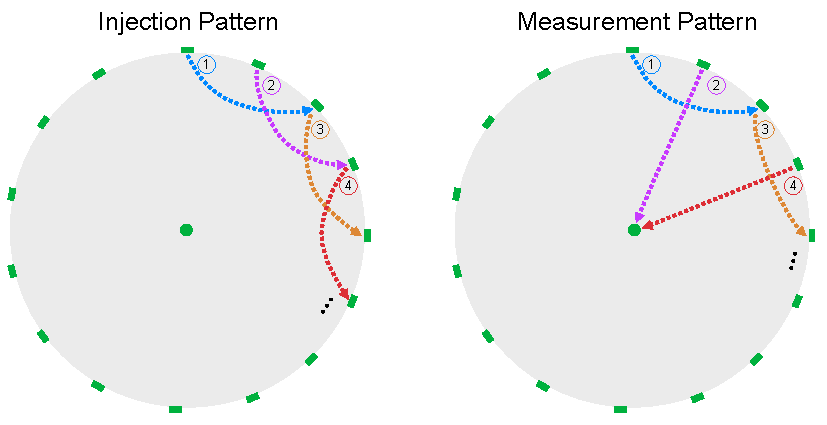
\includegraphics[width=\textwidth]{chapter6-internal_electrodes/imgs/current_injection.pdf}
\caption[Current injection patterns with internal electrodes]{A proposed current injection and measurement pattern for \acrshort{eit} imaging with 2 internal electrodes.
The injection pattern is a typical ``skip 4 '' pattern injecting between every 5\textsuperscript{th} electrode in a square electrode layout and the
measurement pattern replaces every 2\textsuperscript{nd} measurement in the typical method with a measurement between the internal probe and
external rings. Note: this figure does not differentiate between upper and lower electrode planes, but all injections and measurements are done between 
the 2 planes.}
\label{fig:modified_measurement}
\end{figure}

\section{Results}

Reconstructions of the conductive object with and without additive noise are 
shown in \fref{fig:reconstruction_comparison}. With and without additive measurement noise,
all models are able to reconstruct the target object. 
Measurements with internal electrodes appear to reconstruct the target 
closer to the actual size compared to configurations with external electrodes.

\begin{figure}[H]
\centering
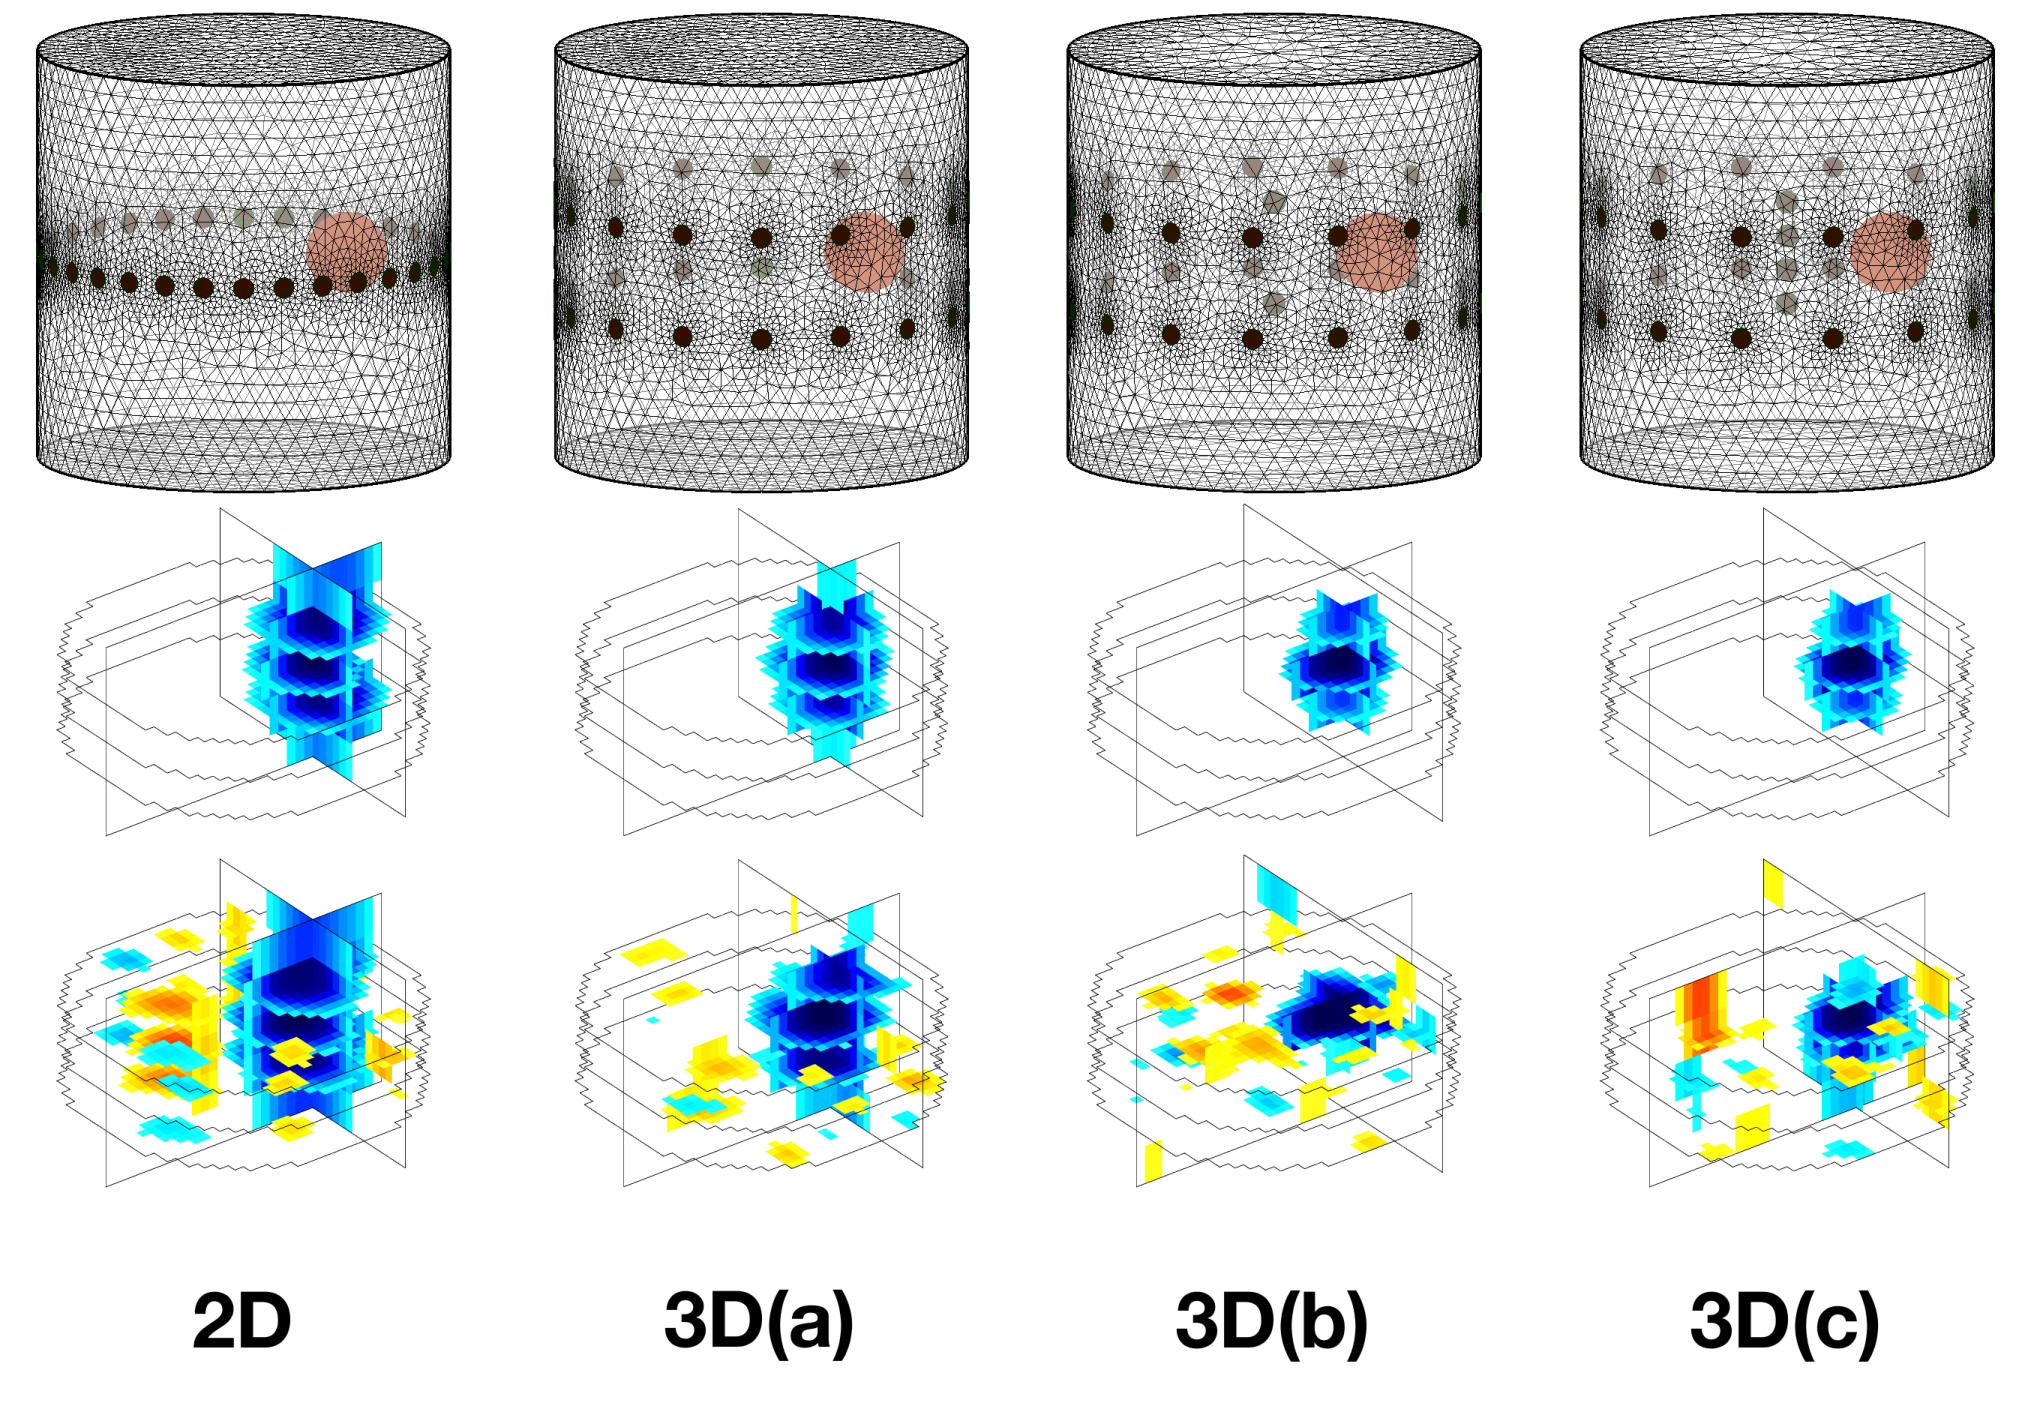
\includegraphics[width=\textwidth]{chapter6-internal_electrodes/imgs/Image_Comparison.pdf}
\caption[Internal electrode simulation reconstructions]{The top row shows reconstructions with no additive noise, and the second row shows reconstructions on measurements with 5dB of
additive noise.}
\label{fig:reconstruction_comparison}
\end{figure}

A 2D arrangements of electrodes is not able to distinguish between 
conductivity changes above and below the electrdes, which contributes to the large
reconstructed area. For this reason it is unusual to display reconstructions 
with a 2D ring of electrode in 3D, but the resulting image helps to visualize the
improvement of 3D electrode arrangements.

\Fref{fig:internal_sensitivity} shows internal sensitivity distribution changes when 
using two and four internal electrodes compared to the
typical 2D and 3D configurations with only external electrodes. 
The highest central sensitivity can be seen when using four internal 
electrodes. This electrode configuration also 
gives a higher sensitivity in between the internal electrodes
and the tank boundary.

\begin{figure}[H]
\centering
%\includegraphics[trim=0 65 0 400,clip,width=\textwidth]{chapter2/imgs/Sensitivity_Comparison_new.pdf}
\includegraphics[width=\textwidth]{chapter6-internal_electrodes/imgs/Sensitivity_Comparison_new.pdf}
\caption[Sensitivity with different internal electrode configurations]{Sensitivity distributions for electrode patterns from left to right: A single 2D electrode plane; 2 electrode planes of 16 electrodes 
each; 2 internal electrodes and 2 external electrode rings of 15 electrodes; 4 internal electrodes arranged between 2 planes of 14 external
electrodes}
\label{fig:internal_sensitivity}
\end{figure}

These results show the expected increased sensitivity in the central regions of the model. 
To further improve internal sensitivity a new
measurement pattern is proposed that uses more measurements between the 
internal probe and peripheral electrodes. 
The sensitivity of the proposed pattern was compared to the sensitivity profile 
of the same configuration using 
the basic ``skip 4'' injection pattern.
Using this injection pattern results show a further increase in sensitivity 
in the internal regions without increasing the measurement
acquisition time. The sensitivity distribution for the new injection pattern 
is pictured in \fref{fig:modified_measurement_sens}.

\begin{figure}[H]
\centering
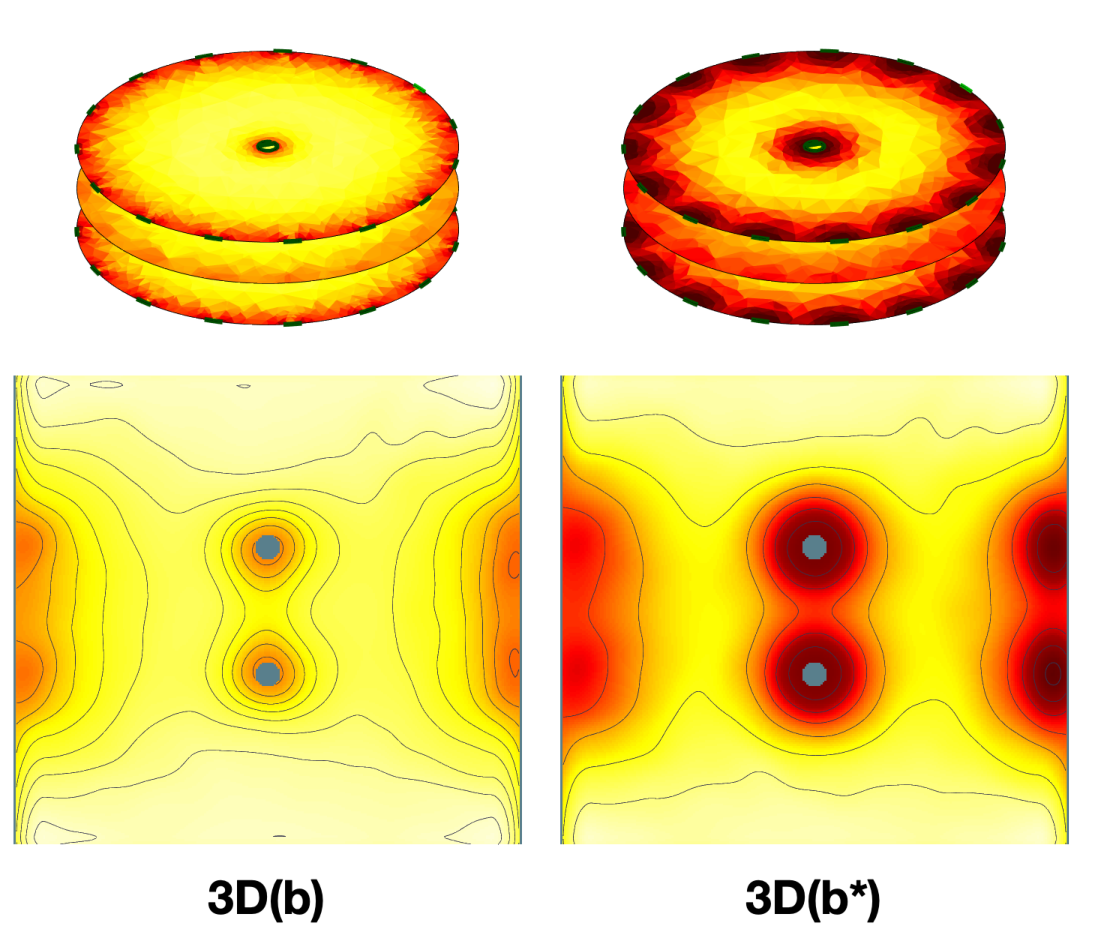
\includegraphics[width=\textwidth]{chapter6-internal_electrodes/imgs/Injection_Comparison.pdf}
\caption[Sensitivity using internal electrodes with modified injection patterns]{A comparison between the sensitivity distributions for a typical ``skip 4'' injection pattern pictured on the left (3D(b)) and 
the modified injection and measurement pattern on the right (3D(b*)).}
\label{fig:modified_measurement_sens}
\end{figure}

\subsection{Sensitivity in an Ovine Model}

A sensitivity comparison was also computed for an ovine model with different 
electrode configurations 
and is shown below in 
\fref{fig:sens_example}. Due to the location of the esophagus in adult sheep
and the distance from the heart
adding internal electrodes resulted 
in a minimal sensitivity decrease in the 
heart region of the model (<1\%), but there is 
a large sensitivity increase in the area immediately surrounding the 
probe.

\begin{figure}[H]
\centering
% Use the following line with your images (pdf preferred)
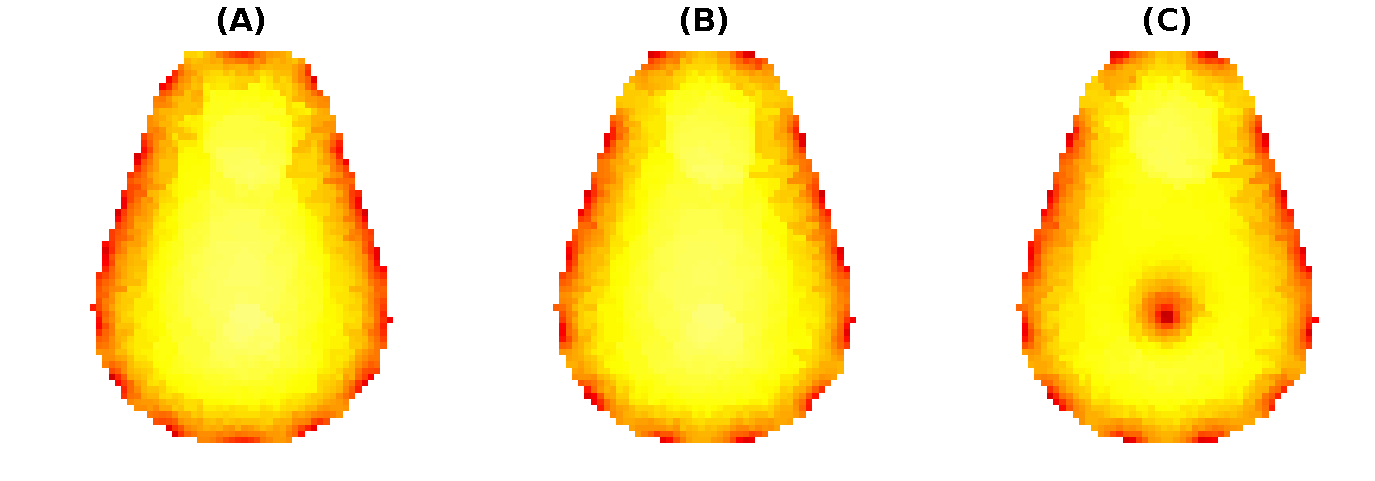
\includegraphics[width=\columnwidth]{chapter6-internal_electrodes/imgs/lamb_sensitivity_profiles.pdf}
\caption[Sensitivity distribution in a lamb model]{\label{fig:sens_example}%
Sensitivity distribution averaged across 10 evenly spaced layers
between the electrode planes in the lamb model for: 
A) 32 external electrodes 
B) 28 external electrodes 
c) 28 external electrodes and 4 internal electrodes.
}
\end{figure}

\section{Discussion}

Based on the simulations presented in this chapter 
internal electrodes were able to increase the sensitivity in 
the central regions of the model. 
Reconstruction in 3D with GREIT was able to accurately 
reconstruct the location of an object in 3D with both 
two and four internal electrodes in the presence of 5 dB 
measurement noise. 

These results align with findings 
from \citeauthorandyear{nasehi_tehrani_evaluation_2012}
who demonstrated that internal electrodes in 2D 
result in a higher reconstruction accuracy and 
a much higher internal sensitivity relative to external configurations.

The presented data validates that the benefits of internal electrodes seen in 2D
are also realizable in 3D, but there is more 
work required to quantify and validate the improvements in real-world settings. 
Additionally reconstructions on a static target with a static electrode probe
are relatively simple. It has been shown that electrode motion and boundary
deformation are major contributing factors to error in EIT 
recordings \parencite{boyle_impact_2011,grychtol_impact_2012}, and this 
has been presented as an additional concern when using internal electrodes
that there is currently no solution for \parencite{nguyen_electrical_2020}.
The following chapter explores this source of error in more detail and 
provides a solution to correct for internal motion.

While the modified current injection pattern increased sensitivity in central
regions of the model, it is not likely feasible for real-world use. 
The majority of commercially available EIT systems use fixed  stimulation and measurement spacing
and would not be able to accommodate this type of measurement. 
Additionally if movement of the internal probe is one of the main sources of artefacts when 
using internal electrodes, it is possible that using the probe for 
more measurements will not improve the reconstructed image.

Sensitively modelling in an ovine model showed a large 
increase in sensitivity surrounding the
internal probe, but no improvement in sensitivity in the heart region.
The ovine model is very different to the human model where 
the heart is much closer to the esophagus. The ovine model may be sufficient 
to analyze the feasibility of internal electrodes for ventilation and lung perfusion imaging, 
but may not be comparable to data collected in humans due to the difference in 
physiology. 

These results serve as a starting point for 3D EIT, demonstrating 
that sensitivity increases  
in the centre of the model when using internal electrodes. 
Four internal electrodes gave the largest increase in internal sensitivity.
The next chapter elaborates on the benefit of internal electrodes
demonstrating reconstruction accuracy in simulations. 

\section{Summary}
Reconstructions using the GREIT algorithm
with internal electrodes on 
an esophageal probe were able to give increased
sensitivity in internal regions. This shows promise for increased 
sensitivity to cardiosynchronous signals 
and may allow better isolation of pulsatile 
motion related to perfusion. 
The following chapter further investigates the impact of motion on internal 
electrodes.